\chapter{Demonstration: Global Illumination}

\section{Results obtained}
\label{ResultsObtained}

\par
The developed application was tested in three different devices:

\begin{itemize}
	\item Samsung Galaxy Fresh Duos GT-S7392
	\item Raspberry Pi 2 Model B
	\item MINIX NEO X8-H PLUS (k200)
\end{itemize}

\begin{table}[H]
	\small
	\centering
	\caption{Devices specifications.}
	\label{specs}
	\hspace*{-2cm}
	\begin{tabular}{|l|l|l|l|l|}
		\hline
		Device&CPU&Cache(L1/L2/L3)&GPU&RAM\\ \hline
		Samsung Galaxy Fresh&1xARM Cortex A9 @1GHz&64KB/Unknown&1xBroadcom VideoCore IV&512MB\\ \hline
		Raspberry Pi 2 Model B&4xARM Cortex A7 @900MHz&64KB/1MB&1xBroadcom VideoCore IV&1GB\\ \hline
		MINIX NEO X8 PLUS&4xARM Cortex A9 @2.0GHz&64KB/Unknown&8xMali-450 MP&2GB\\ \hline
	\end{tabular}
\end{table}

\par
As you can see in the table \ref{specs}, the application has been tested on a few devices.
Unfortunately, it was only possible to test it on one mobile device, the Samsung Galaxy Fresh Duos GT-S7392.
This device is a low-end smartphone with a low-end single core CPU.

\par
It was also possible to test it on two different computers that are portable and even smaller than a common laptop.
The Raspberry Pi 2 Model B and the MINIX NEO X8-H PLUS which are devices with the Android operating system installed.

\par
In order to assess the performance of the ray tracer, it was tested with three different scenes and with Whitted and Path Tracing shaders.
One large scene with some hundred of thousands triangles, one moderate with few thousand of triangles and one small scene with just some dozens triangles.

\par
The large scene used for testing was the conference scene, as illustrated in figure \ref{scene_conference}.
This scene consists of 331179 triangles and has two area lights in form of triangles.

\begin{figure}[H]
	\centering
	\caption{Illustration of conference scene, rendered with shader Whitted in MobileRT.}
	\label{scene_conference}
	\includegraphics[keepaspectratio,scale=0.5]{Scene_Conference.png}
\end{figure}

The medium scene used for testing was the Porsche 911 GT2 scene, as illustrated in figure \ref{scene_porsche}.
This scene consists of 22017 triangles and has two area lights in form of triangles.

\begin{figure}[H]
	\centering
	\caption{Illustration of Porsche 911 GT2 scene, rendered with shader Whitted in MobileRT.}
	\label{scene_porsche}
	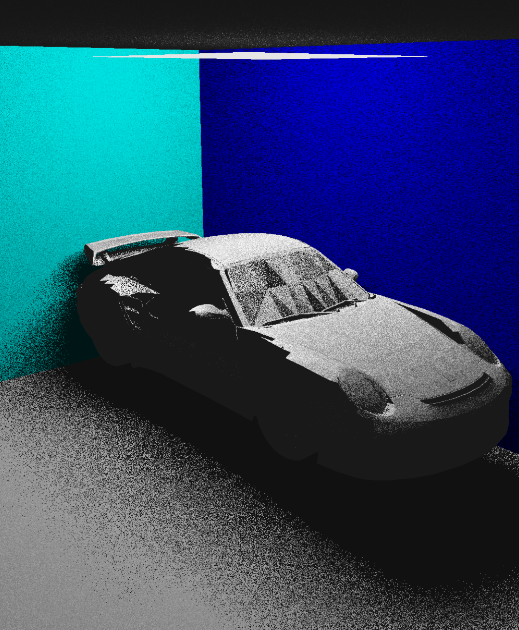
\includegraphics[keepaspectratio,scale=0.5]{Scene_Porsche.png}
\end{figure}

The small scene used for testing was the Cornell Box scene, as illustrated in figure \ref{scene_cornellbox}.
This scene consists of 34 triangles and has two area lights in form of triangles.

\begin{figure}[H]
	\centering
	\caption{Illustration of Cornell Box scene, rendered with shader Whitted in MobileRT.}
	\label{scene_cornellbox}
	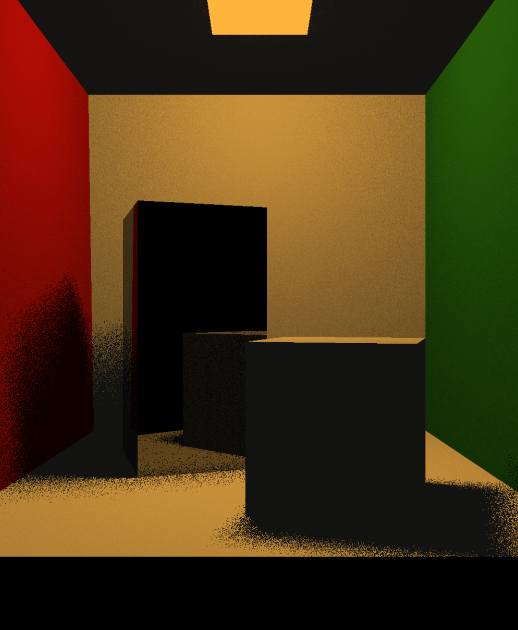
\includegraphics[keepaspectratio,scale=0.5]{Scene_CornellBox.png}
\end{figure}

\par
All of the used scenes models were downloaded from
\url{http://casual-effects.com/data/index.html}  (\cite{McGuire2017Data}).

\subsection{Whitted Shader}

\subsubsection{Samsung Galaxy Fresh Duos GT-S7392}

\begin{figure}[H]
	\begin{tikzpicture}
	\begin{axis}[
	legend style={at={(1.05,1.00)},anchor=north west},
	axis lines = left,
	xlabel = \#threads,
	ylabel = time (ms),
	xtick={0,1,2,3,4},
	ytick={0,1,...,10},
	width=0.75\textwidth,
	]
	\addplot [
	color=red,
	mark=*,
	dashed,
	] plot coordinates {
		(0,0.0)
		(1,1.0)
		(2,1.0)
		(3,1.0)
		(4,1.0)
	};
	\addlegendentry{BVH}
	\addplot [
	color=black,
	mark=*,
	dashed,
	] plot coordinates {
		(0,0.0)
		(1,1.0)
		(2,1.0)
		(3,1.0)
		(4,1.0)
	};
	\addlegendentry{Regular Grid}
	\addplot [
	color=blue,
	mark=*,
	dashed,
	] plot coordinates {
		(0,0.0)
		(1,1.0)
		(2,1.0)
		(3,1.0)
		(4,1.0)
	};
	\addlegendentry{Naive}
	\label{graph:SamsungTime}
	\end{axis}
	\end{tikzpicture}
	\caption{Time in the scene 1}
\end{figure}

\begin{figure}[H]
\begin{tikzpicture}
\begin{axis}[
legend style={at={(1.05,1.00)},anchor=north west},
axis lines = left,
xlabel = \#threads,
ylabel = speedup,
xtick={0,1,2,3,4},
ytick={0,1,...,10},
width=0.75\textwidth,
]
\addplot [
color=red,
mark=*,
dashed,
] plot coordinates {
	(0,0.0)
	(1,1.0)
	(2,1.0)
	(3,1.0)
	(4,1.0)
};
\addlegendentry{BVH}
\addplot [
color=black,
mark=*,
dashed,
] plot coordinates {
	(0,0.0)
	(1,1.0)
	(2,1.0)
	(3,1.0)
	(4,1.0)
};
\addlegendentry{Regular Grid}
\addplot [
color=blue,
mark=*,
dashed,
] plot coordinates {
	(0,0.0)
	(1,1.0)
	(2,1.0)
	(3,1.0)
	(4,1.0)
};
\addlegendentry{Naive}
\label{graph:SamsungSpeedup}
\end{axis}
\end{tikzpicture}
\caption{Speedup in the scene 1}
\end{figure}

\begin{figure}[H]
	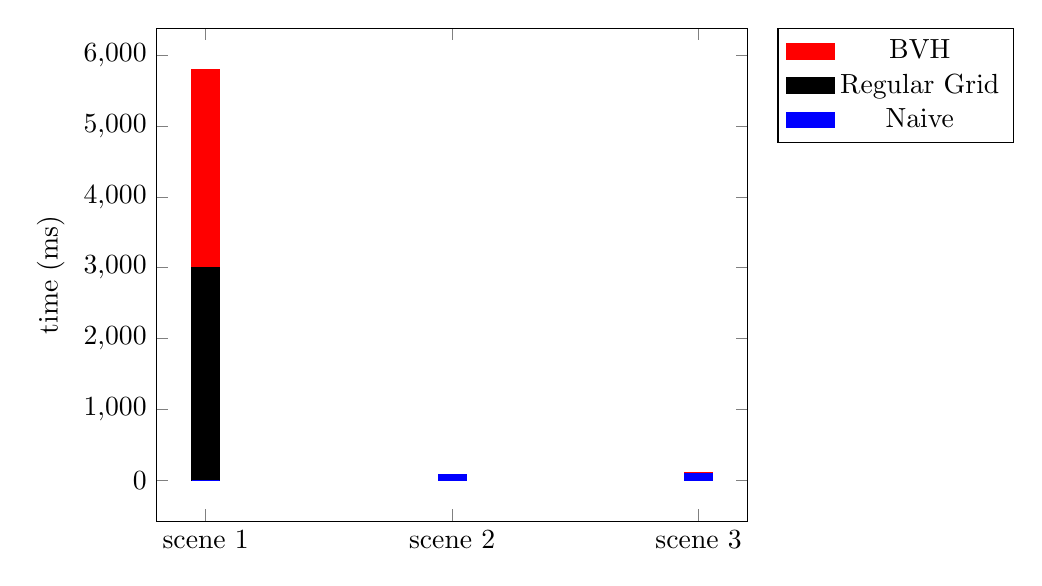
\begin{tikzpicture}
	\begin{axis}[
	legend style={at={(1.05,1.00)},anchor=north west},
	ylabel = time (ms),
	symbolic x coords={scene 1, scene 2, scene 3},
	xtick=data,
	width=0.75\textwidth,
	]
	\addplot[ybar,fill=red,color=red,area legend] coordinates {
		(scene 1,   0)
		(scene 1,   5800)
		(scene 2,  	85)
		(scene 3,   105)
	};
	\addlegendentry{BVH}
	\addplot[ybar,fill=black,color=black,area legend] coordinates {
		(scene 1,   0)
		(scene 1,   3000)
		(scene 2,  	80)
		(scene 3,   99)
	};
	\addlegendentry{Regular Grid}
	\addplot[ybar,fill=blue,color=blue,area legend] coordinates {
		(scene 1,   0)
		(scene 1,   0)
		(scene 2,  	77)
		(scene 3,   91)
	};
	\addlegendentry{Naive}
	\end{axis}
	\label{graph:SamsungConstruct}
	\end{tikzpicture}
	\caption{Time to construct accelerators in Samsung Galaxy smart phone}
\end{figure}

\begin{figure}[H]
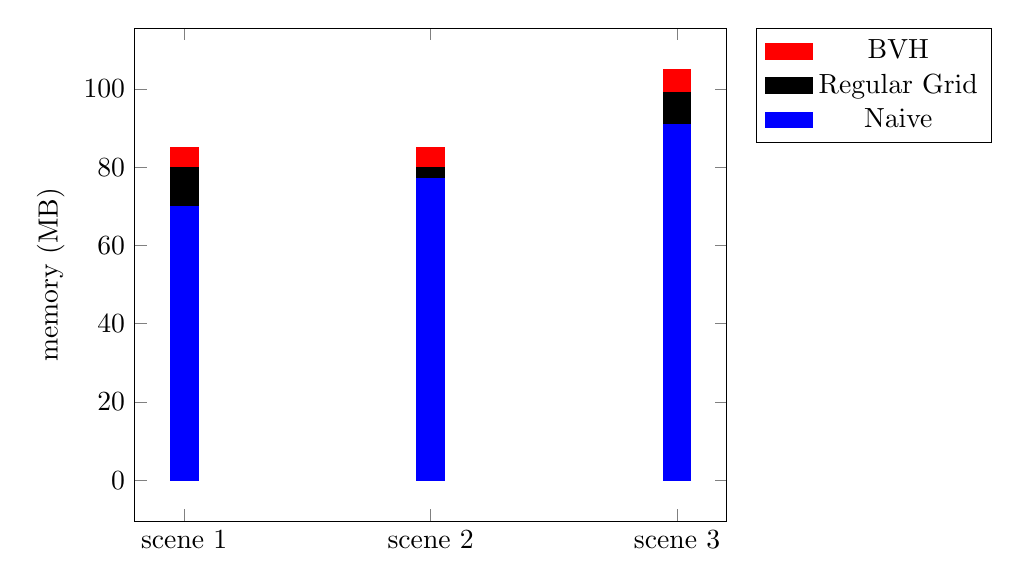
\begin{tikzpicture}
\begin{axis}[
legend style={at={(1.05,1.00)},anchor=north west},
ylabel = memory (MB),
symbolic x coords={scene 1, scene 2, scene 3},
xtick=data,
width=0.75\textwidth,
]
\addplot[ybar,fill=red,color=red,area legend] coordinates {
	(scene 1,   0)
	(scene 1,   85)
	(scene 2,  	85)
	(scene 3,   105)
};
\addlegendentry{BVH}
\addplot[ybar,fill=black,color=black,area legend] coordinates {
	(scene 1,   0)
	(scene 1,   80)
	(scene 2,  	80)
	(scene 3,   99)
};
\addlegendentry{Regular Grid}
\addplot[ybar,fill=blue,color=blue,area legend] coordinates {
	(scene 1,   0)
	(scene 1,   70)
	(scene 2,  	77)
	(scene 3,   91)
};
\addlegendentry{Naive}
\end{axis}
\label{graph:SamsungMemory}
\end{tikzpicture}
\caption{Memory usage in the Samsung Galaxy smart phone}
\end{figure}

\subsubsection{Raspberry Pi 2 Model B}

\begin{figure}[H]
	\begin{tikzpicture}
	\begin{axis}[
	legend style={at={(1.05,1.00)},anchor=north west},
	axis lines = left,
	xlabel = \#threads,
	ylabel = time (ms),
	xtick={0,1,2,3,4},
	ytick={0,1,...,10},
	width=0.75\textwidth,
	]
	\addplot [
	color=red,
	mark=*,
	dashed,
	] plot coordinates {
		(0,0.0)
		(1,1.0)
		(2,1.0)
		(3,1.0)
		(4,1.0)
	};
	\addlegendentry{BVH}
	\addplot [
	color=black,
	mark=*,
	dashed,
	] plot coordinates {
		(0,0.0)
		(1,1.0)
		(2,1.0)
		(3,1.0)
		(4,1.0)
	};
	\addlegendentry{Regular Grid}
	\addplot [
	color=blue,
	mark=*,
	dashed,
	] plot coordinates {
		(0,0.0)
		(1,1.0)
		(2,1.0)
		(3,1.0)
		(4,1.0)
	};
	\addlegendentry{Naive}
	\label{graph:RaspberryTime}
	\end{axis}
	\end{tikzpicture}
\end{figure}

\begin{figure}[H]
\begin{tikzpicture}
\begin{axis}[
legend style={at={(1.05,1.00)},anchor=north west},
axis lines = left,
xlabel = \#threads,
ylabel = speedup,
xtick={0,1,2,3,4},
ytick={0,1,...,10},
width=0.75\textwidth,
]
\addplot [
color=red,
mark=*,
dashed,
] plot coordinates {
	(0,0.0)
	(1,1.0)
	(2,1.0)
	(3,1.0)
	(4,1.0)
};
\addlegendentry{BVH}
\addplot [
color=black,
mark=*,
dashed,
] plot coordinates {
	(0,0.0)
	(1,1.0)
	(2,1.0)
	(3,1.0)
	(4,1.0)
};
\addlegendentry{Regular Grid}
\addplot [
color=blue,
mark=*,
dashed,
] plot coordinates {
	(0,0.0)
	(1,1.0)
	(2,1.0)
	(3,1.0)
	(4,1.0)
};
\addlegendentry{Naive}
\label{graph:RaspberrySpeedup}
\end{axis}
\end{tikzpicture}
\end{figure}

\begin{figure}[H]
	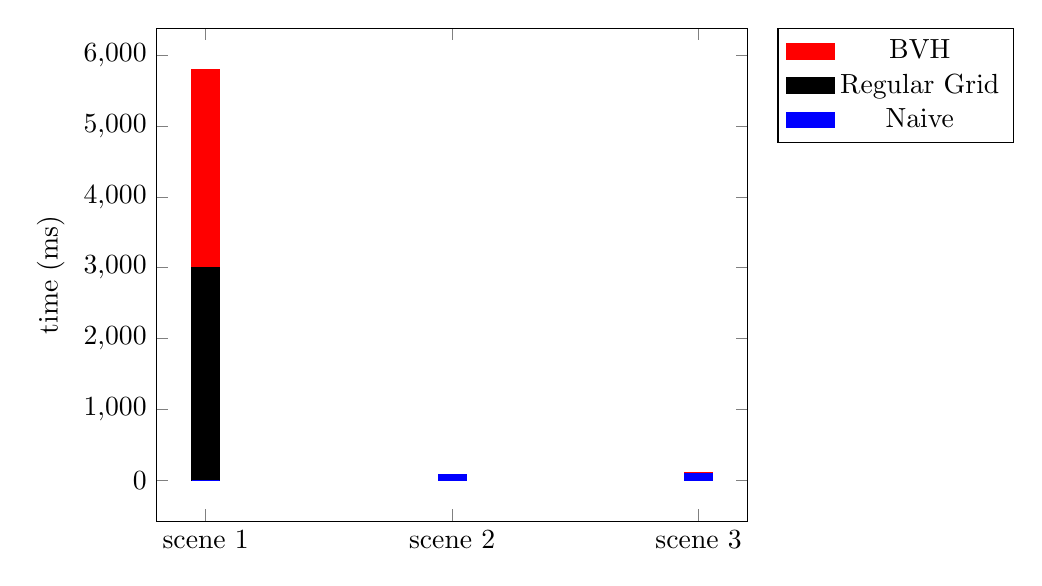
\begin{tikzpicture}
	\begin{axis}[
	legend style={at={(1.05,1.00)},anchor=north west},
	ylabel = time (ms),
	symbolic x coords={scene 1, scene 2, scene 3},
	xtick=data,
	width=0.75\textwidth,
	]
	\addplot[ybar,fill=red,color=red,area legend] coordinates {
		(scene 1,   0)
		(scene 1,   5800)
		(scene 2,  	85)
		(scene 3,   105)
	};
	\addlegendentry{BVH}
	\addplot[ybar,fill=black,color=black,area legend] coordinates {
		(scene 1,   0)
		(scene 1,   3000)
		(scene 2,  	80)
		(scene 3,   99)
	};
	\addlegendentry{Regular Grid}
	\addplot[ybar,fill=blue,color=blue,area legend] coordinates {
		(scene 1,   0)
		(scene 1,   0)
		(scene 2,  	77)
		(scene 3,   91)
	};
	\addlegendentry{Naive}
	\end{axis}
	\label{graph:RaspberryConstruct}
	\end{tikzpicture}
	\caption{Time to construct accelerators in the Raspberry Pi 2 Model B}
\end{figure}

\begin{figure}[H]
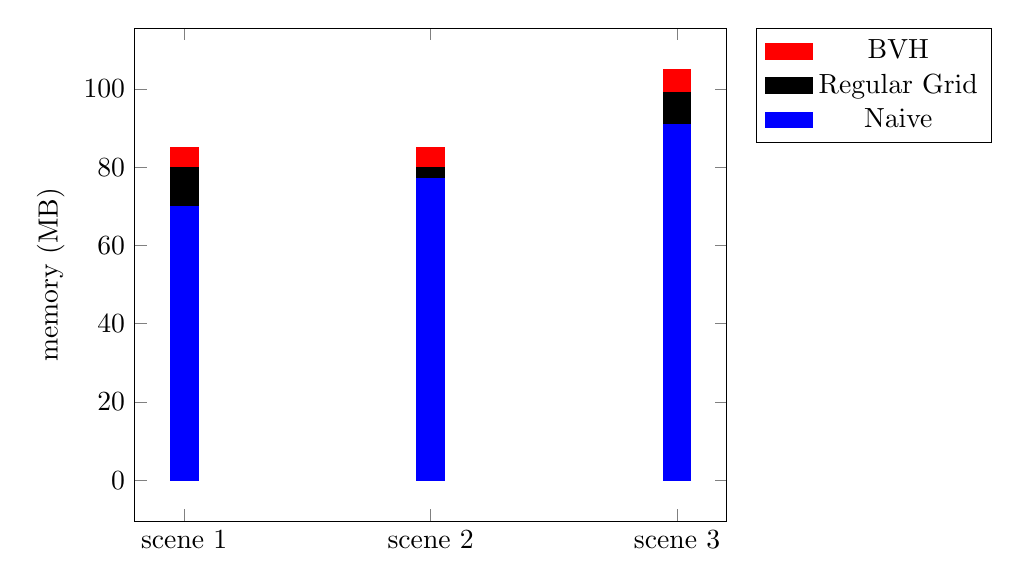
\begin{tikzpicture}
\begin{axis}[
legend style={at={(1.05,1.00)},anchor=north west},
ylabel = memory (MB),
symbolic x coords={scene 1, scene 2, scene 3},
xtick=data,
width=0.75\textwidth,
]
\addplot[ybar,fill=red,color=red,area legend] coordinates {
	(scene 1,   0)
	(scene 1,   85)
	(scene 2,  	85)
	(scene 3,   105)
};
\addlegendentry{BVH}
\addplot[ybar,fill=black,color=black,area legend] coordinates {
	(scene 1,   0)
	(scene 1,   80)
	(scene 2,  	80)
	(scene 3,   99)
};
\addlegendentry{Regular Grid}
\addplot[ybar,fill=blue,color=blue,area legend] coordinates {
	(scene 1,   0)
	(scene 1,   70)
	(scene 2,  	77)
	(scene 3,   91)
};
\addlegendentry{Naive}
\end{axis}
\label{graph:RaspberryMemory}
\end{tikzpicture}
\caption{Memory usage in the Raspberry Pi 2 Model B}
\end{figure}


\subsubsection{MINIX NEO X8-H PLUS}

\begin{figure}[H]
	\begin{tikzpicture}
	\begin{axis}[
	legend style={at={(1.05,1.00)},anchor=north west},
	axis lines = left,
	xlabel = \#threads,
	ylabel = time (ms),
	xtick={0,1,2,3,4},
	ytick={0,1,...,10},
	width=0.75\textwidth,
	]
	\addplot [
	color=red,
	mark=*,
	dashed,
	] plot coordinates {
		(0,0.0)
		(1,1.0)
		(2,1.0)
		(3,1.0)
		(4,1.0)
	};
	\addlegendentry{BVH}
	\addplot [
	color=black,
	mark=*,
	dashed,
	] plot coordinates {
		(0,0.0)
		(1,1.0)
		(2,1.0)
		(3,1.0)
		(4,1.0)
	};
	\addlegendentry{Regular Grid}
	\addplot [
	color=blue,
	mark=*,
	dashed,
	] plot coordinates {
		(0,0.0)
		(1,1.0)
		(2,1.0)
		(3,1.0)
		(4,1.0)
	};
	\addlegendentry{Naive}
	\label{graph:MinixTime}
	\end{axis}
	\end{tikzpicture}
\end{figure}

\begin{figure}[H]
\begin{tikzpicture}
\begin{axis}[
legend style={at={(1.05,1.00)},anchor=north west},
axis lines = left,
xlabel = \#threads,
ylabel = speedup,
xtick={0,1,2,3,4},
ytick={0,1,...,10},
width=0.75\textwidth,
]
\addplot [
color=red,
mark=*,
dashed,
] plot coordinates {
	(0,0.0)
	(1,1.0)
	(2,1.0)
	(3,1.0)
	(4,1.0)
};
\addlegendentry{BVH}
\addplot [
color=black,
mark=*,
dashed,
] plot coordinates {
	(0,0.0)
	(1,1.0)
	(2,1.0)
	(3,1.0)
	(4,1.0)
};
\addlegendentry{Regular Grid}
\addplot [
color=blue,
mark=*,
dashed,
] plot coordinates {
	(0,0.0)
	(1,1.0)
	(2,1.0)
	(3,1.0)
	(4,1.0)
};
\addlegendentry{Naive}
\label{graph:MinixSpeedup}
\end{axis}
\end{tikzpicture}
\end{figure}

\begin{figure}[H]
	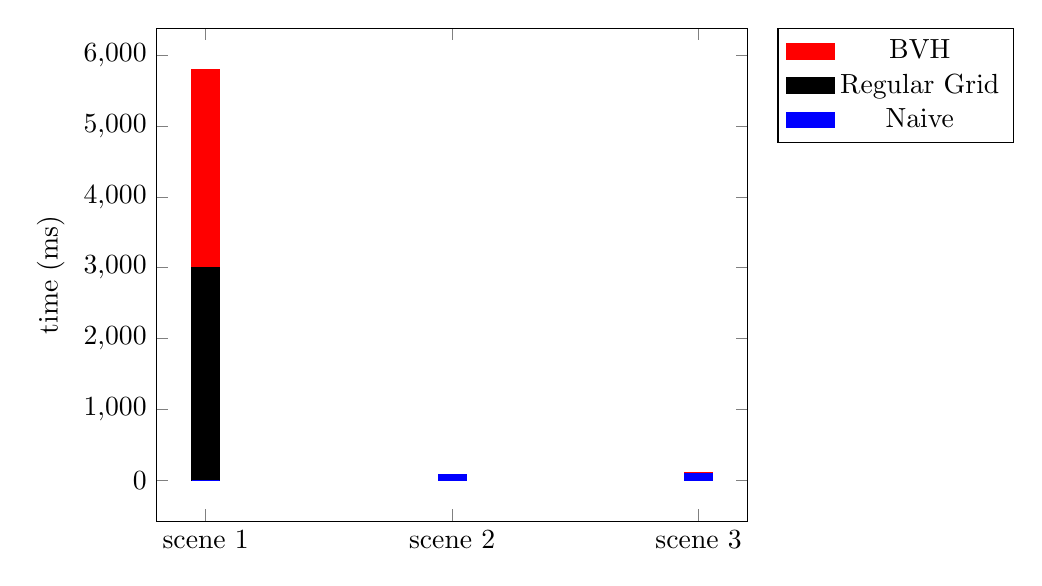
\begin{tikzpicture}
	\begin{axis}[
	legend style={at={(1.05,1.00)},anchor=north west},
	ylabel = time (ms),
	symbolic x coords={scene 1, scene 2, scene 3},
	xtick=data,
	width=0.75\textwidth,
	]
	\addplot[ybar,fill=red,color=red,area legend] coordinates {
		(scene 1,   0)
		(scene 1,   5800)
		(scene 2,  	85)
		(scene 3,   105)
	};
	\addlegendentry{BVH}
	\addplot[ybar,fill=black,color=black,area legend] coordinates {
		(scene 1,   0)
		(scene 1,   3000)
		(scene 2,  	80)
		(scene 3,   99)
	};
	\addlegendentry{Regular Grid}
	\addplot[ybar,fill=blue,color=blue,area legend] coordinates {
		(scene 1,   0)
		(scene 1,   0)
		(scene 2,  	77)
		(scene 3,   91)
	};
	\addlegendentry{Naive}
	\end{axis}
	\label{graph:MinixConstruct}
	\end{tikzpicture}
	\caption{Time to construct accelerators in the MINIX NEO X8-H PLUS}
\end{figure}

\begin{figure}[H]
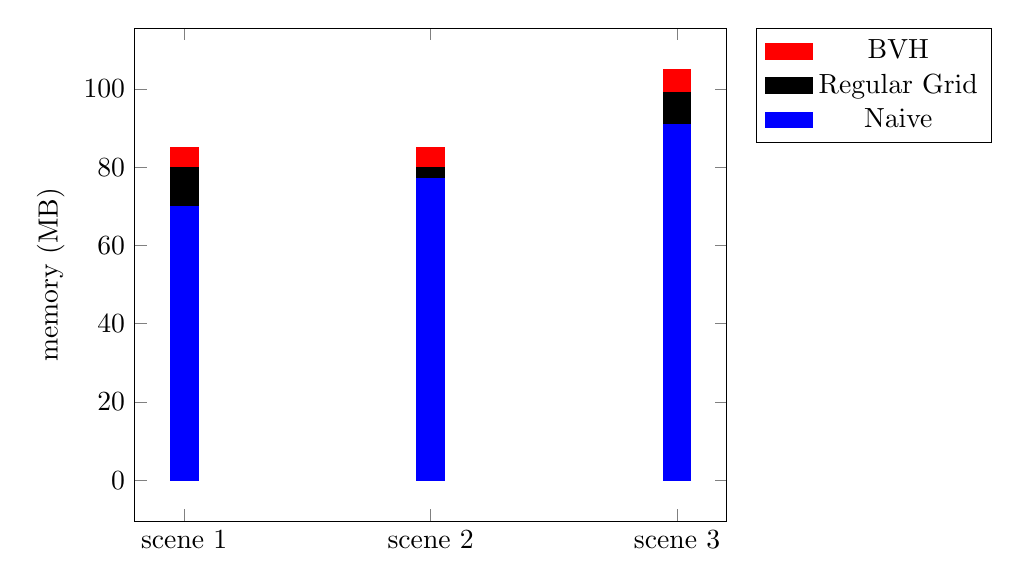
\begin{tikzpicture}
\begin{axis}[
legend style={at={(1.05,1.00)},anchor=north west},
ylabel = memory (MB),
symbolic x coords={scene 1, scene 2, scene 3},
xtick=data,
width=0.75\textwidth,
]
\addplot[ybar,fill=red,color=red,area legend,width=4.30\textwidth] coordinates {
	(scene 1,   0)
	(scene 1,   85)
	(scene 2,  	85)
	(scene 3,   105)
};
\addlegendentry{BVH}
\addplot[ybar,fill=black,color=black,area legend] coordinates {
	(scene 1,   0)
	(scene 1,   80)
	(scene 2,  	80)
	(scene 3,   99)
};
\addlegendentry{Regular Grid}
\addplot[ybar,fill=blue,color=blue,area legend] coordinates {
	(scene 1,   0)
	(scene 1,   70)
	(scene 2,  	77)
	(scene 3,   91)
};
\addlegendentry{Naive}
\end{axis}
\label{graph:MinixMemory}
\end{tikzpicture}
\caption{Memory usage in the MINIX NEO X8-H PLUS}
\end{figure}

\subsection{Path Tracing Shader}

\subsubsection{Samsung Galaxy Fresh Duos GT-S7392}

\begin{figure}[H]
	\begin{tikzpicture}
	\begin{axis}[
	legend style={at={(1.05,1.00)},anchor=north west},
	axis lines = left,
	xlabel = \#threads,
	ylabel = time (ms),
	xtick={0,1,2,3,4},
	ytick={0,1,...,10},
	width=0.75\textwidth,
	]
	\addplot [
	color=red,
	mark=*,
	dashed,
	] plot coordinates {
		(0,0.0)
		(1,1.0)
		(2,1.0)
		(3,1.0)
		(4,1.0)
	};
	\addlegendentry{BVH}
	\addplot [
	color=black,
	mark=*,
	dashed,
	] plot coordinates {
		(0,0.0)
		(1,1.0)
		(2,1.0)
		(3,1.0)
		(4,1.0)
	};
	\addlegendentry{Regular Grid}
	\addplot [
	color=blue,
	mark=*,
	dashed,
	] plot coordinates {
		(0,0.0)
		(1,1.0)
		(2,1.0)
		(3,1.0)
		(4,1.0)
	};
	\addlegendentry{Naive}
	\label{graph:SamsungTime}
	\end{axis}
	\end{tikzpicture}
	\caption{Time in the scene 1}
\end{figure}

\begin{figure}[H]
	\begin{tikzpicture}
	\begin{axis}[
	legend style={at={(1.05,1.00)},anchor=north west},
	axis lines = left,
	xlabel = \#threads,
	ylabel = speedup,
	xtick={0,1,2,3,4},
	ytick={0,1,...,10},
	width=0.75\textwidth,
	]
	\addplot [
	color=red,
	mark=*,
	dashed,
	] plot coordinates {
		(0,0.0)
		(1,1.0)
		(2,1.0)
		(3,1.0)
		(4,1.0)
	};
	\addlegendentry{BVH}
	\addplot [
	color=black,
	mark=*,
	dashed,
	] plot coordinates {
		(0,0.0)
		(1,1.0)
		(2,1.0)
		(3,1.0)
		(4,1.0)
	};
	\addlegendentry{Regular Grid}
	\addplot [
	color=blue,
	mark=*,
	dashed,
	] plot coordinates {
		(0,0.0)
		(1,1.0)
		(2,1.0)
		(3,1.0)
		(4,1.0)
	};
	\addlegendentry{Naive}
	\label{graph:SamsungSpeedup}
	\end{axis}
	\end{tikzpicture}
	\caption{Speedup in the scene 1}
\end{figure}

\begin{figure}[H]
	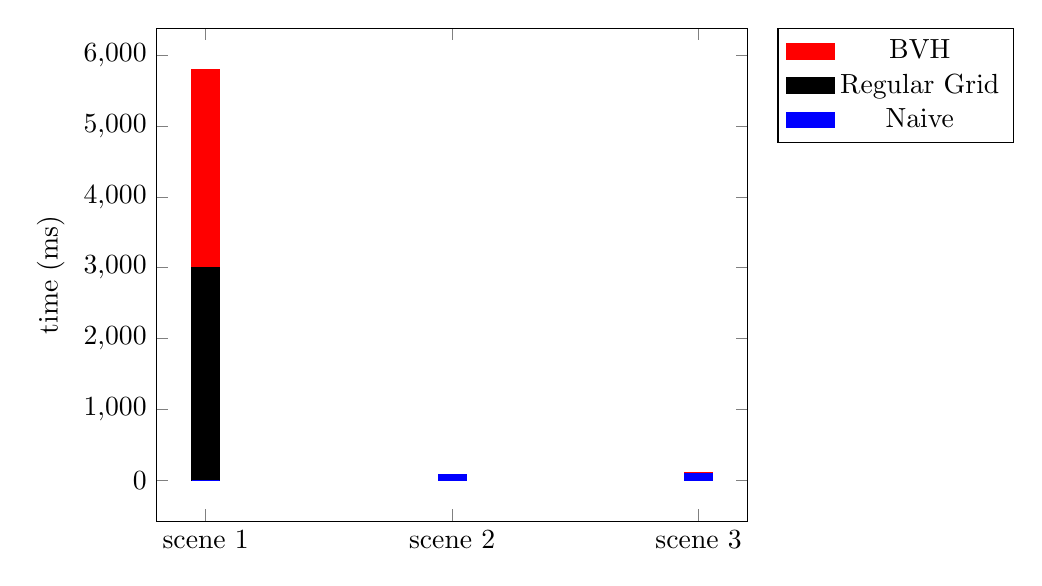
\begin{tikzpicture}
	\begin{axis}[
	legend style={at={(1.05,1.00)},anchor=north west},
	ylabel = time (ms),
	symbolic x coords={scene 1, scene 2, scene 3},
	xtick=data,
	width=0.75\textwidth,
	]
	\addplot[ybar,fill=red,color=red,area legend] coordinates {
		(scene 1,   0)
		(scene 1,   5800)
		(scene 2,  	85)
		(scene 3,   105)
	};
	\addlegendentry{BVH}
	\addplot[ybar,fill=black,color=black,area legend] coordinates {
		(scene 1,   0)
		(scene 1,   3000)
		(scene 2,  	80)
		(scene 3,   99)
	};
	\addlegendentry{Regular Grid}
	\addplot[ybar,fill=blue,color=blue,area legend] coordinates {
		(scene 1,   0)
		(scene 1,   0)
		(scene 2,  	77)
		(scene 3,   91)
	};
	\addlegendentry{Naive}
	\end{axis}
	\label{graph:SamsungConstruct}
	\end{tikzpicture}
	\caption{Time to construct accelerators in Samsung Galaxy smart phone}
\end{figure}

\begin{figure}[H]
	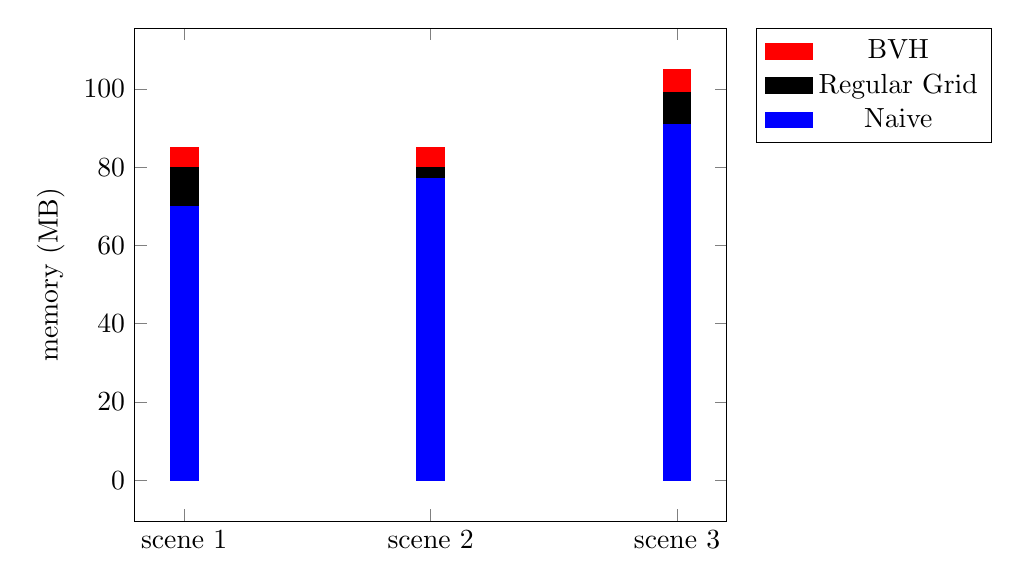
\begin{tikzpicture}
	\begin{axis}[
	legend style={at={(1.05,1.00)},anchor=north west},
	ylabel = memory (MB),
	symbolic x coords={scene 1, scene 2, scene 3},
	xtick=data,
	width=0.75\textwidth,
	]
	\addplot[ybar,fill=red,color=red,area legend] coordinates {
		(scene 1,   0)
		(scene 1,   85)
		(scene 2,  	85)
		(scene 3,   105)
	};
	\addlegendentry{BVH}
	\addplot[ybar,fill=black,color=black,area legend] coordinates {
		(scene 1,   0)
		(scene 1,   80)
		(scene 2,  	80)
		(scene 3,   99)
	};
	\addlegendentry{Regular Grid}
	\addplot[ybar,fill=blue,color=blue,area legend] coordinates {
		(scene 1,   0)
		(scene 1,   70)
		(scene 2,  	77)
		(scene 3,   91)
	};
	\addlegendentry{Naive}
	\end{axis}
	\label{graph:SamsungMemory}
	\end{tikzpicture}
	\caption{Memory usage in the Samsung Galaxy smart phone}
\end{figure}

\subsubsection{Raspberry Pi 2 Model B}

\begin{figure}[H]
	\begin{tikzpicture}
	\begin{axis}[
	legend style={at={(1.05,1.00)},anchor=north west},
	axis lines = left,
	xlabel = \#threads,
	ylabel = time (ms),
	xtick={0,1,2,3,4},
	ytick={0,1,...,10},
	width=0.75\textwidth,
	]
	\addplot [
	color=red,
	mark=*,
	dashed,
	] plot coordinates {
		(0,0.0)
		(1,1.0)
		(2,1.0)
		(3,1.0)
		(4,1.0)
	};
	\addlegendentry{BVH}
	\addplot [
	color=black,
	mark=*,
	dashed,
	] plot coordinates {
		(0,0.0)
		(1,1.0)
		(2,1.0)
		(3,1.0)
		(4,1.0)
	};
	\addlegendentry{Regular Grid}
	\addplot [
	color=blue,
	mark=*,
	dashed,
	] plot coordinates {
		(0,0.0)
		(1,1.0)
		(2,1.0)
		(3,1.0)
		(4,1.0)
	};
	\addlegendentry{Naive}
	\label{graph:RaspberryTime}
	\end{axis}
	\end{tikzpicture}
\end{figure}

\begin{figure}[H]
	\begin{tikzpicture}
	\begin{axis}[
	legend style={at={(1.05,1.00)},anchor=north west},
	axis lines = left,
	xlabel = \#threads,
	ylabel = speedup,
	xtick={0,1,2,3,4},
	ytick={0,1,...,10},
	width=0.75\textwidth,
	]
	\addplot [
	color=red,
	mark=*,
	dashed,
	] plot coordinates {
		(0,0.0)
		(1,1.0)
		(2,1.0)
		(3,1.0)
		(4,1.0)
	};
	\addlegendentry{BVH}
	\addplot [
	color=black,
	mark=*,
	dashed,
	] plot coordinates {
		(0,0.0)
		(1,1.0)
		(2,1.0)
		(3,1.0)
		(4,1.0)
	};
	\addlegendentry{Regular Grid}
	\addplot [
	color=blue,
	mark=*,
	dashed,
	] plot coordinates {
		(0,0.0)
		(1,1.0)
		(2,1.0)
		(3,1.0)
		(4,1.0)
	};
	\addlegendentry{Naive}
	\label{graph:RaspberrySpeedup}
	\end{axis}
	\end{tikzpicture}
\end{figure}

\begin{figure}[H]
	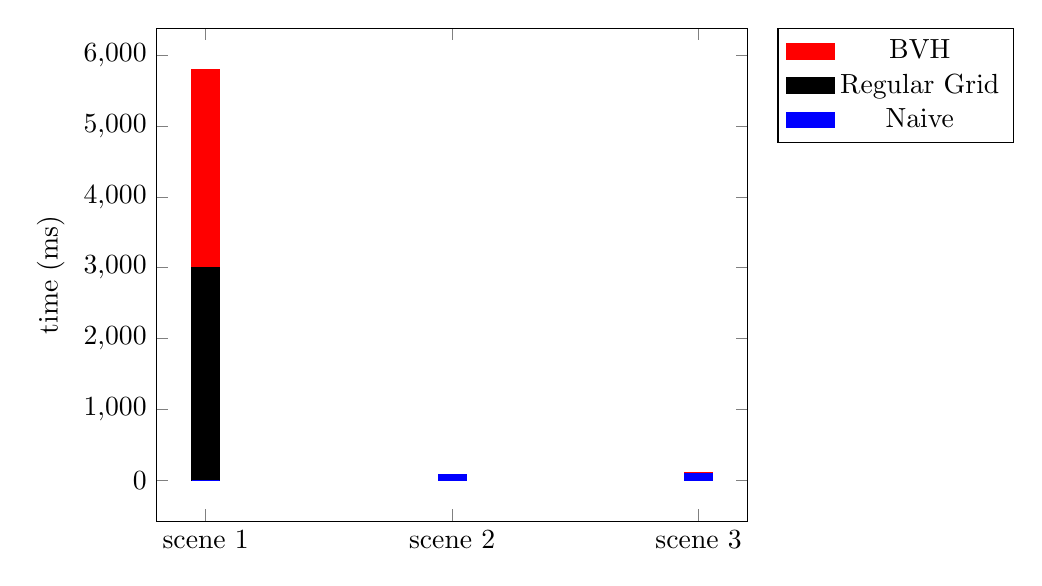
\begin{tikzpicture}
	\begin{axis}[
	legend style={at={(1.05,1.00)},anchor=north west},
	ylabel = time (ms),
	symbolic x coords={scene 1, scene 2, scene 3},
	xtick=data,
	width=0.75\textwidth,
	]
	\addplot[ybar,fill=red,color=red,area legend] coordinates {
		(scene 1,   0)
		(scene 1,   5800)
		(scene 2,  	85)
		(scene 3,   105)
	};
	\addlegendentry{BVH}
	\addplot[ybar,fill=black,color=black,area legend] coordinates {
		(scene 1,   0)
		(scene 1,   3000)
		(scene 2,  	80)
		(scene 3,   99)
	};
	\addlegendentry{Regular Grid}
	\addplot[ybar,fill=blue,color=blue,area legend] coordinates {
		(scene 1,   0)
		(scene 1,   0)
		(scene 2,  	77)
		(scene 3,   91)
	};
	\addlegendentry{Naive}
	\end{axis}
	\label{graph:RaspberryConstruct}
	\end{tikzpicture}
	\caption{Time to construct accelerators in the Raspberry Pi 2 Model B}
\end{figure}

\begin{figure}[H]
	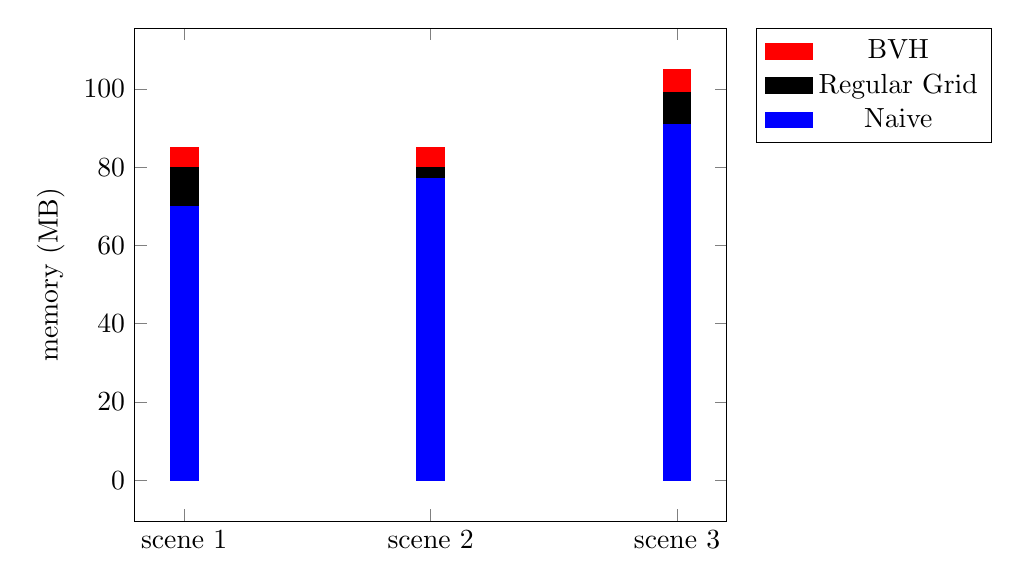
\begin{tikzpicture}
	\begin{axis}[
	legend style={at={(1.05,1.00)},anchor=north west},
	ylabel = memory (MB),
	symbolic x coords={scene 1, scene 2, scene 3},
	xtick=data,
	width=0.75\textwidth,
	]
	\addplot[ybar,fill=red,color=red,area legend] coordinates {
		(scene 1,   0)
		(scene 1,   85)
		(scene 2,  	85)
		(scene 3,   105)
	};
	\addlegendentry{BVH}
	\addplot[ybar,fill=black,color=black,area legend] coordinates {
		(scene 1,   0)
		(scene 1,   80)
		(scene 2,  	80)
		(scene 3,   99)
	};
	\addlegendentry{Regular Grid}
	\addplot[ybar,fill=blue,color=blue,area legend] coordinates {
		(scene 1,   0)
		(scene 1,   70)
		(scene 2,  	77)
		(scene 3,   91)
	};
	\addlegendentry{Naive}
	\end{axis}
	\label{graph:RaspberryMemory}
	\end{tikzpicture}
	\caption{Memory usage in the Raspberry Pi 2 Model B}
\end{figure}


\subsubsection{MINIX NEO X8-H PLUS}

\begin{figure}[H]
	\begin{tikzpicture}
	\begin{axis}[
	legend style={at={(1.05,1.00)},anchor=north west},
	axis lines = left,
	xlabel = \#threads,
	ylabel = time (ms),
	xtick={0,1,2,3,4},
	ytick={0,1,...,10},
	width=0.75\textwidth,
	]
	\addplot [
	color=red,
	mark=*,
	dashed,
	] plot coordinates {
		(0,0.0)
		(1,1.0)
		(2,1.0)
		(3,1.0)
		(4,1.0)
	};
	\addlegendentry{BVH}
	\addplot [
	color=black,
	mark=*,
	dashed,
	] plot coordinates {
		(0,0.0)
		(1,1.0)
		(2,1.0)
		(3,1.0)
		(4,1.0)
	};
	\addlegendentry{Regular Grid}
	\addplot [
	color=blue,
	mark=*,
	dashed,
	] plot coordinates {
		(0,0.0)
		(1,1.0)
		(2,1.0)
		(3,1.0)
		(4,1.0)
	};
	\addlegendentry{Naive}
	\label{graph:MinixTime}
	\end{axis}
	\end{tikzpicture}
\end{figure}

\begin{figure}[H]
	\begin{tikzpicture}
	\begin{axis}[
	legend style={at={(1.05,1.00)},anchor=north west},
	axis lines = left,
	xlabel = \#threads,
	ylabel = speedup,
	xtick={0,1,2,3,4},
	ytick={0,1,...,10},
	width=0.75\textwidth,
	]
	\addplot [
	color=red,
	mark=*,
	dashed,
	] plot coordinates {
		(0,0.0)
		(1,1.0)
		(2,1.0)
		(3,1.0)
		(4,1.0)
	};
	\addlegendentry{BVH}
	\addplot [
	color=black,
	mark=*,
	dashed,
	] plot coordinates {
		(0,0.0)
		(1,1.0)
		(2,1.0)
		(3,1.0)
		(4,1.0)
	};
	\addlegendentry{Regular Grid}
	\addplot [
	color=blue,
	mark=*,
	dashed,
	] plot coordinates {
		(0,0.0)
		(1,1.0)
		(2,1.0)
		(3,1.0)
		(4,1.0)
	};
	\addlegendentry{Naive}
	\label{graph:MinixSpeedup}
	\end{axis}
	\end{tikzpicture}
\end{figure}

\begin{figure}[H]
	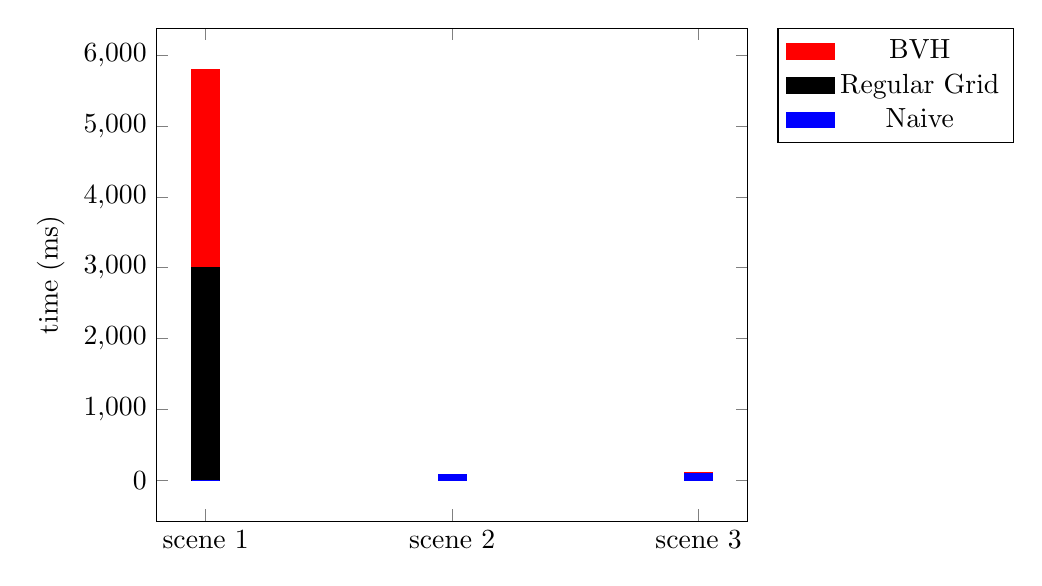
\begin{tikzpicture}
	\begin{axis}[
	legend style={at={(1.05,1.00)},anchor=north west},
	ylabel = time (ms),
	symbolic x coords={scene 1, scene 2, scene 3},
	xtick=data,
	width=0.75\textwidth,
	]
	\addplot[ybar,fill=red,color=red,area legend] coordinates {
		(scene 1,   0)
		(scene 1,   5800)
		(scene 2,  	85)
		(scene 3,   105)
	};
	\addlegendentry{BVH}
	\addplot[ybar,fill=black,color=black,area legend] coordinates {
		(scene 1,   0)
		(scene 1,   3000)
		(scene 2,  	80)
		(scene 3,   99)
	};
	\addlegendentry{Regular Grid}
	\addplot[ybar,fill=blue,color=blue,area legend] coordinates {
		(scene 1,   0)
		(scene 1,   0)
		(scene 2,  	77)
		(scene 3,   91)
	};
	\addlegendentry{Naive}
	\end{axis}
	\label{graph:MinixConstruct}
	\end{tikzpicture}
	\caption{Time to construct accelerators in the MINIX NEO X8-H PLUS}
\end{figure}

\begin{figure}[H]
	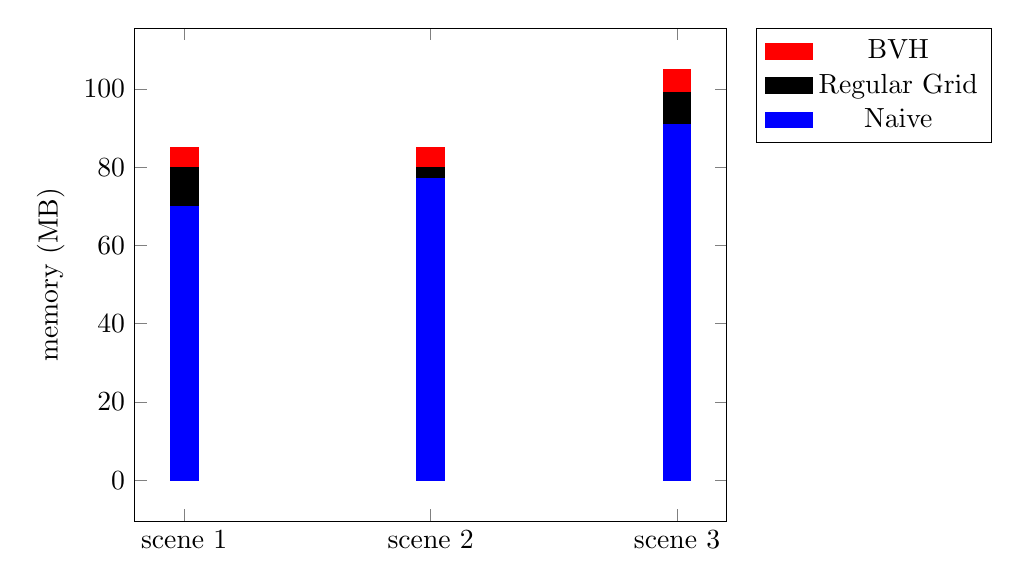
\begin{tikzpicture}
	\begin{axis}[
	legend style={at={(1.05,1.00)},anchor=north west},
	ylabel = memory (MB),
	symbolic x coords={scene 1, scene 2, scene 3},
	xtick=data,
	width=0.75\textwidth,
	]
	\addplot[ybar,fill=red,color=red,area legend,width=4.30\textwidth] coordinates {
		(scene 1,   0)
		(scene 1,   85)
		(scene 2,  	85)
		(scene 3,   105)
	};
	\addlegendentry{BVH}
	\addplot[ybar,fill=black,color=black,area legend] coordinates {
		(scene 1,   0)
		(scene 1,   80)
		(scene 2,  	80)
		(scene 3,   99)
	};
	\addlegendentry{Regular Grid}
	\addplot[ybar,fill=blue,color=blue,area legend] coordinates {
		(scene 1,   0)
		(scene 1,   70)
		(scene 2,  	77)
		(scene 3,   91)
	};
	\addlegendentry{Naive}
	\end{axis}
	\label{graph:MinixMemory}
	\end{tikzpicture}
	\caption{Memory usage in the MINIX NEO X8-H PLUS}
\end{figure}

\section{Comparison with Android CPU Raytracer (\cite{Android_CPU_Raytracer})}

\par
Comparison ...